% Requires in the preamble:
% \usepackage{amsmath,amssymb}
% \usepackage{tikz,pgfplots}
% \pgfplotsset{compat=1.18}

\chapter{Technology Notes}
\label{app:technology-notes}

Calculus is older than computers, but modern calculus practice is full of screens:
graphing calculators, spreadsheets, computer algebra systems, numerical solvers, and
short programs.

These tools are useful because calculus is full of processes:

\[
\text{zoom in on a graph},
\qquad
\text{iterate Newton's method},
\qquad
\text{add a Riemann sum},
\qquad
\text{plot partial sums},
\qquad
\text{compare Taylor polynomials}.
\]

A computer can do thousands of arithmetic steps before a person finishes writing the
first line.  That speed is powerful.  It also creates a new responsibility.

\[
\boxed{
\text{Technology should extend mathematical judgment, not replace it.}
}
\]

This appendix gives practical notes for using technology in this book.  The examples use
generic calculator language and simple Python code.  The exact syntax of a particular
device or app may differ, but the mathematical habits are the same.

\section{Graphing windows}
\label{appsec:graphing-windows}

A graph on a screen is not the graph itself.

It is a sampled picture of part of the graph, drawn in a chosen rectangle:

\[
x_{\min}\le x\le x_{\max},
\qquad
y_{\min}\le y\le y_{\max}.
\]

Anything outside that rectangle is invisible.  Anything between sampled points may be
missed.  A good graphing window reveals structure.  A poor window hides it.

\subsection{A window is a mathematical choice}
\label{appsubsec:window-choice}

Consider

\[
f(x)=x^3-6x.
\]

In the small window

\[
-1\le x\le1,
\qquad
-6\le y\le6,
\]

the graph looks mostly like a decreasing curve.  In the wider window

\[
-3\le x\le3,
\qquad
-12\le y\le12,
\]

we see the full cubic shape: rising, falling, then rising again.

\begin{figure}[h]
\centering
\begin{minipage}{0.47\textwidth}
\centering
\begin{tikzpicture}
\begin{axis}[
    width=\textwidth,
    height=0.76\textwidth,
    xmin=-1, xmax=1,
    ymin=-6, ymax=6,
    axis lines=middle,
    xlabel={\(x\)},
    ylabel={\(y\)},
    xtick={-1,0,1},
    ytick={-6,0,6},
    grid=both,
    grid style={line width=.1pt, draw=gray!25},
    title={small window}
]
\addplot[very thick, domain=-1:1, samples=120] {x^3-6*x};
\end{axis}
\end{tikzpicture}
\end{minipage}
\hfill
\begin{minipage}{0.47\textwidth}
\centering
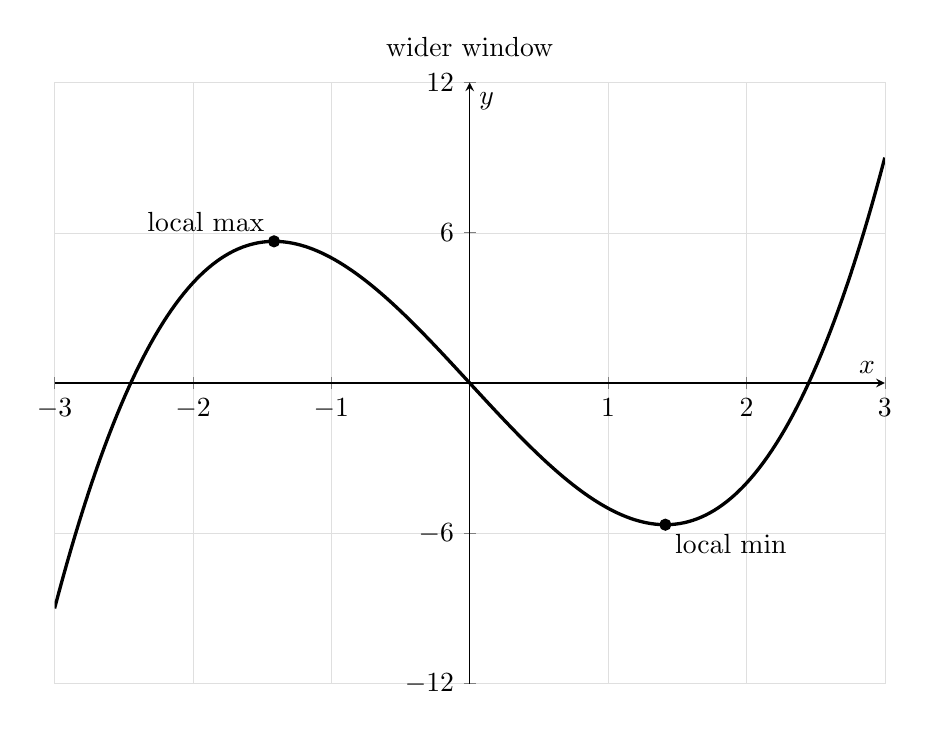
\begin{tikzpicture}
\begin{axis}[
    width=\textwidth,
    height=0.76\textwidth,
    xmin=-3, xmax=3,
    ymin=-12, ymax=12,
    axis lines=middle,
    xlabel={\(x\)},
    ylabel={\(y\)},
    xtick={-3,-2,-1,0,1,2,3},
    ytick={-12,-6,0,6,12},
    grid=both,
    grid style={line width=.1pt, draw=gray!25},
    title={wider window}
]
\addplot[very thick, domain=-3:3, samples=200] {x^3-6*x};
\addplot[only marks, mark=*] coordinates {(-1.414,5.657) (1.414,-5.657)};
\node[anchor=south east] at (axis cs:-1.414,5.657) {local max};
\node[anchor=north west] at (axis cs:1.414,-5.657) {local min};
\end{axis}
\end{tikzpicture}
\end{minipage}
\caption{The same function can tell a different visual story in different windows.}
\label{fig:technology-window-cubic}
\end{figure}

The function did not change.  The picture changed.

\begin{quote}
\textbf{Window habit.}
Before trusting a graph, change the window.

Try a smaller window, a larger window, and a window centered on important points:
zeros, critical points, endpoints, and possible asymptotes.
\end{quote}

\subsection{A graph can hide a hole}
\label{appsubsec:graph-can-hide-hole}

Technology often draws connected pixels.  That can hide a missing point.

Consider

\[
g(x)=\frac{x^2-1}{x-1}.
\]

Algebraically,

\[
x^2-1=(x-1)(x+1).
\]

So for

\[
x\neq1,
\]

we have

\[
g(x)=x+1.
\]

But the original function is undefined at

\[
x=1.
\]

So the correct graph is the line

\[
y=x+1
\]

with a hole at

\[
(1,2).
\]

A graphing device may draw only the line and may not show the hole.

\begin{figure}[h]
\centering
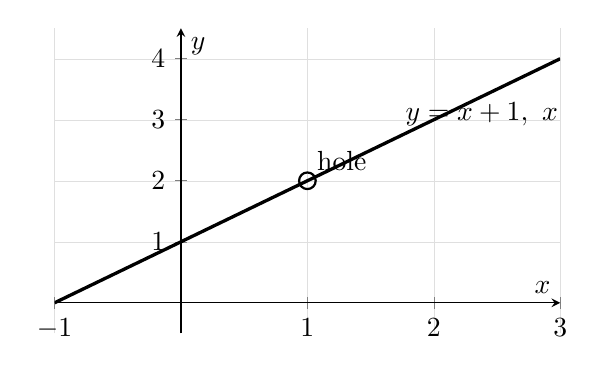
\begin{tikzpicture}
\begin{axis}[
    width=0.66\textwidth,
    height=0.45\textwidth,
    xmin=-1, xmax=3,
    ymin=-0.5, ymax=4.5,
    axis lines=middle,
    xlabel={\(x\)},
    ylabel={\(y\)},
    xtick={-1,0,1,2,3},
    ytick={0,1,2,3,4},
    grid=both,
    grid style={line width=.1pt, draw=gray!25},
]
\addplot[very thick, domain=-1:3, samples=2] {x+1};
\addplot[only marks, mark=o, mark size=3pt, thick] coordinates {(1,2)};
\node[anchor=south west] at (axis cs:1,2) {hole};
\node[anchor=west] at (axis cs:1.7,3.1) {\(y=x+1,\ x\neq1\)};
\end{axis}
\end{tikzpicture}
\caption{A plotted line may hide the fact that the original formula is undefined at \(x=1\).}
\label{fig:technology-hidden-hole}
\end{figure}

This is not a failure of technology.  It is a reminder that a graphing tool cannot know
which features matter unless we ask mathematically.

\[
\boxed{
\text{The domain is part of the function.}
}
\]

\subsection{A graph can hide a sharp feature}
\label{appsubsec:graph-can-hide-sharp-feature}

A graphing device samples finitely many points.  If important behavior occurs between
sampled points, the plotted graph may miss it.

For example,

\[
f(x)=\sin(100x)
\]

oscillates rapidly.  A coarse plot may connect sampled points in a way that looks much
less oscillatory than the true function.

\begin{figure}[h]
\centering
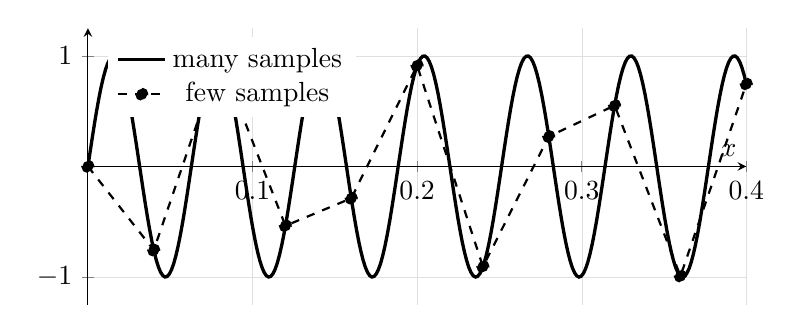
\begin{tikzpicture}
\begin{axis}[
    width=0.82\textwidth,
    height=0.42\textwidth,
    xmin=0, xmax=0.4,
    ymin=-1.25, ymax=1.25,
    axis lines=middle,
    xlabel={\(x\)},
    ylabel={},
    xtick={0,0.1,0.2,0.3,0.4},
    ytick={-1,0,1},
    grid=both,
    grid style={line width=.1pt, draw=gray!25},
    legend style={draw=none, at={(0.03,0.97)}, anchor=north west}
]
\addplot[very thick, domain=0:0.4, samples=300] {sin(deg(100*x))};
\addlegendentry{many samples}
\addplot[thick, dashed, mark=*] coordinates {
    (0,0)
    (0.04,{sin(deg(4))})
    (0.08,{sin(deg(8))})
    (0.12,{sin(deg(12))})
    (0.16,{sin(deg(16))})
    (0.20,{sin(deg(20))})
    (0.24,{sin(deg(24))})
    (0.28,{sin(deg(28))})
    (0.32,{sin(deg(32))})
    (0.36,{sin(deg(36))})
    (0.40,{sin(deg(40))})
};
\addlegendentry{few samples}
\end{axis}
\end{tikzpicture}
\caption{Sampling too few points can give a misleading picture of a rapidly changing function.}
\label{fig:technology-sampling-oscillation}
\end{figure}

This matters in calculus because derivatives, roots, local extrema, asymptotes, and
oscillations may all be small or narrow enough to be missed in a first plot.

\subsection{A graphing checklist}
\label{appsubsec:graphing-checklist}

When using a graphing tool, ask these questions.

\begin{center}
\renewcommand{\arraystretch}{1.5}
\begin{tabular}{p{0.36\textwidth}|p{0.48\textwidth}}
\textbf{question} & \textbf{why it matters} \\ \hline
What is the domain? & A plotted curve may hide holes or forbidden inputs. \\

What window am I using? & Important behavior may lie outside the viewing rectangle. \\

Does the graph have asymptotes? & Connecting across an asymptote can produce false lines. \\

Have I zoomed in near zeros and critical points? & Local behavior may be invisible at a large scale. \\

Have I zoomed out? & End behavior and global shape may be invisible at a small scale. \\

Does algebra confirm the picture? & Factoring, derivatives, and limits reveal features a plot may miss.
\end{tabular}
\end{center}

\begin{quote}
\textbf{Graphing principle.}
A graph is evidence.  It is not a proof.

Use it to form guesses.  Use algebra, calculus, and domain information to check them.
\end{quote}

\section{Numerical precision and roundoff}
\label{appsec:numerical-precision-roundoff}

A real number can have infinitely many decimal places.  A machine stores only finitely
many digits.

That difference is small in many calculations and large in some.

Calculus cares about small errors, so we must know how numerical errors enter.

\subsection{Exact arithmetic and floating-point arithmetic}
\label{appsubsec:exact-and-floating-point}

In exact mathematics,

\[
\frac{1}{3}
\]

is exactly one third.

In decimal floating-point arithmetic, it must be stored approximately:

\[
0.333333333333\ldots
\]

with only finitely many digits.

Similarly,

\[
\sqrt2
\]

is an exact number in mathematics, but a decimal approximation in a calculator.

A computer typically stores a number in scientific notation, roughly like

\[
\pm d_1.d_2d_3\cdots d_k\times 10^m,
\]

where only finitely many digits are kept.  The exact storage system depends on the
machine and software, but the main idea is universal:

\[
\boxed{
\text{Most real numbers are rounded when stored.}
}
\]

\begin{quote}
\textbf{Roundoff error.}
\emph{Roundoff error} is the error introduced when a real number is replaced by a
nearby machine-representable number.
\end{quote}

This does not make computation unreliable.  It means computation must be interpreted
with error in mind.

\subsection{Subtraction can magnify relative error}
\label{appsubsec:cancellation}

The most dangerous basic operation is often subtraction of nearly equal numbers.

Suppose a calculator stores the two numbers

\[
1.0000001
\qquad\text{and}\qquad
1.0000000
\]

with limited precision.  Their difference is

\[
0.0000001.
\]

If each input has small rounding error, the difference may have a large relative error,
because the true answer is very small.

This problem is called \emph{cancellation}.

Calculus produces cancellation often.  The difference quotient

\[
\frac{f(x+h)-f(x)}{h}
\]

subtracts two nearby function values when \(h\) is small.  If \(h\) is too small on a
computer, roundoff error can overwhelm the improvement we expected from taking a
smaller interval.

\paragraph{Example: a numerically unstable expression.}
Consider

\[
Q(x)=\frac{\sqrt{1+x}-1}{x}
\]

for \(x\) near \(0\).

Mathematically, rationalize:

\[
\frac{\sqrt{1+x}-1}{x}
\cdot
\frac{\sqrt{1+x}+1}{\sqrt{1+x}+1}
=
\frac{1}{\sqrt{1+x}+1},
\qquad x\neq0.
\]

So for \(x\neq0\),

\[
Q(x)=\frac{1}{\sqrt{1+x}+1}.
\]

As \(x\to0\),

\[
Q(x)\to \frac12.
\]

The original form subtracts two nearby numbers:

\[
\sqrt{1+x}
\quad\text{and}\quad
1.
\]

The rationalized form avoids that subtraction.  Near \(x=0\), it is usually more stable
numerically.

\[
\boxed{
\frac{\sqrt{1+x}-1}{x}
\quad\text{and}\quad
\frac{1}{\sqrt{1+x}+1}
}
\]

are algebraically equivalent for \(x\neq0\), but not equally safe for numerical
evaluation.

\begin{quote}
\textbf{Numerical algebra habit.}
Algebraic simplification is not only for exact answers.  It can also make numerical
answers more stable.
\end{quote}

\subsection{Roundoff versus truncation}
\label{appsubsec:roundoff-vs-truncation}

Many numerical methods have two different kinds of error.

\begin{center}
\renewcommand{\arraystretch}{1.6}
\begin{tabular}{p{0.24\textwidth}|p{0.60\textwidth}}
\textbf{error type} & \textbf{meaning} \\ \hline
Truncation error &
The error from replacing an infinite or limiting process by a finite one. \\

Roundoff error &
The error from storing and operating with finitely many digits.
\end{tabular}
\end{center}

\paragraph{Example: derivative approximation.}
To approximate \(f'(a)\), we might use

\[
\frac{f(a+h)-f(a)}{h}.
\]

If \(h\) is large, the secant slope may be a poor approximation to the tangent slope.
That is truncation error.

If \(h\) is extremely small, then \(f(a+h)\) and \(f(a)\) may be almost equal as stored
numbers.  Their subtraction may lose important digits.  That is roundoff error.

So making \(h\) smaller is not always better on a machine.

\begin{quote}
\textbf{Computing warning.}
In exact mathematics,

\[
h\to0
\]

is the right idea.

In floating-point computation, taking \(h\) too small can make the numerical result
worse.
\end{quote}

\subsection{Residuals and step sizes}
\label{appsubsec:residuals-step-sizes}

When an algorithm produces an approximate answer, do not ask only:

\[
\text{Did the program stop?}
\]

Ask:

\[
\text{Why did it stop?}
\]

For root-finding, two common checks are:

\[
|f(x_n)| \quad \text{and} \quad |x_n-x_{n-1}|.
\]

The number \(|f(x_n)|\) is a \emph{residual}.  It tells how close the function value is to
zero.

The number \(|x_n-x_{n-1}|\) is a step size.  It tells how much the approximate root
changed in the last step.

Both can matter.

A small step size alone does not prove that \(f(x_n)\) is small.  An algorithm might be
stuck.

A small residual alone does not always prove the root is known accurately.  If the graph
is very flat or very steep, residual size and input error can behave differently.

\begin{quote}
\textbf{Numerical stopping habit.}
For iterative methods, record at least:

\[
x_n,\qquad f(x_n),\qquad |x_n-x_{n-1}|.
\]

A good computation leaves a trail.
\end{quote}

\section{Calculator and CAS syntax}
\label{appsec:calculator-cas-syntax}

A calculator or computer algebra system must parse what you type.  It does not read
mathematical intention.  Parentheses, multiplication signs, and mode settings matter.

\[
\boxed{
\text{Most technology errors in calculus are syntax errors or interpretation errors.}
}
\]

\subsection{Common syntax translations}
\label{appsubsec:common-syntax-translations}

Different tools use different syntax.  The following table gives common patterns.

\begin{center}
\renewcommand{\arraystretch}{1.65}
\begin{tabular}{c|c|c}
\textbf{mathematics} & \textbf{common calculator/CAS style} & \textbf{Python style} \\ \hline
\(x^2\) & \texttt{x\string^2} or \texttt{x**2} & \texttt{x**2} \\
\(2x\) & \texttt{2*x} & \texttt{2*x} \\
\(\sqrt{x}\) & \texttt{sqrt(x)} & \texttt{sqrt(x)} or \texttt{math.sqrt(x)} \\
\(\sin x\) & \texttt{sin(x)} & \texttt{sin(x)} or \texttt{math.sin(x)} \\
\(e^x\) & \texttt{exp(x)} & \texttt{exp(x)} or \texttt{math.exp(x)} \\
\(\ln x\) & \texttt{ln(x)} or \texttt{log(x)} & \texttt{log(x)} or \texttt{math.log(x)} \\
\(\pi\) & \texttt{pi} or a \(\pi\) key & \texttt{pi} or \texttt{math.pi} \\
\(|x|\) & \texttt{abs(x)} & \texttt{abs(x)}
\end{tabular}
\end{center}

Always check the syntax of the tool you are using.  In Python, for example,

\[
x^2
\]

is not exponentiation in ordinary numerical code.  Exponentiation is

\[
\texttt{x**2}.
\]

\subsection{Parentheses are part of the mathematics}
\label{appsubsec:parentheses-syntax}

The expression

\[
\frac{1}{x+1}
\]

should be typed as

\[
\texttt{1/(x+1)}.
\]

If we type

\[
\texttt{1/x+1},
\]

the machine reads

\[
\frac1x+1,
\]

which is different.

Similarly,

\[
\sin(2x)
\]

should be typed with the multiplication and parentheses:

\[
\texttt{sin(2*x)}.
\]

\begin{center}
\renewcommand{\arraystretch}{1.6}
\begin{tabular}{c|c|c}
\textbf{intended expression} & \textbf{safe input} & \textbf{common wrong input} \\ \hline
\(\displaystyle \frac{1}{x+1}\) &
\texttt{1/(x+1)} &
\texttt{1/x+1} \\

\(\displaystyle \frac{x+2}{x-3}\) &
\texttt{(x+2)/(x-3)} &
\texttt{x+2/x-3} \\

\(\sin(2x)\) &
\texttt{sin(2*x)} &
\texttt{sin2x} \\

\(e^{-x^2}\) &
\texttt{exp(-x**2)} &
\texttt{exp(-x)**2}
\end{tabular}
\end{center}

The last line is especially important:

\[
e^{-x^2}
\neq
(e^{-x})^2.
\]

Indeed,

\[
(e^{-x})^2=e^{-2x}.
\]

\subsection{Radians versus degrees}
\label{appsubsec:radians-vs-degrees}

Calculus uses radians.

The derivative formula

\[
\frac{d}{dx}\sin x=\cos x
\]

is true when \(x\) is measured in radians.  If a calculator is in degree mode, numerical
experiments with derivatives of trigonometric functions will not match the calculus
formulas.

For example, in radians,

\[
\sin\left(\frac{\pi}{6}\right)=\frac12.
\]

In degree mode,

\[
\sin(30)=\frac12.
\]

Both statements can be true in their own systems.  The problem happens when the mode
and the input do not match.

\begin{quote}
\textbf{Trig mode habit.}
Before using technology with sine, cosine, tangent, inverse trigonometric functions,
or polar graphs, check that the angle mode matches the problem.

In this book, use radians unless degrees are explicitly stated.
\end{quote}

\subsection{Exact and approximate answers}
\label{appsubsec:exact-approximate-cas}

A computer algebra system may give exact answers, approximate answers, or both.

For example, it might return

\[
\frac{\sqrt2}{2}
\]

or

\[
0.7071067812.
\]

Both represent the same number, but they serve different purposes.

Exact form is usually better for algebra and proof.  Decimal form is often better for
measurement, numerical comparison, and plotting.

\begin{center}
\renewcommand{\arraystretch}{1.5}
\begin{tabular}{p{0.38\textwidth}|p{0.46\textwidth}}
\textbf{use exact form when} & \textbf{use decimal form when} \\ \hline
simplifying symbols & reporting a measured quantity \\
checking identities & comparing numerical sizes quickly \\
finding exact roots or areas & plotting or simulating \\
proving a formula & estimating error numerically
\end{tabular}
\end{center}

\subsection{CAS answers need interpretation}
\label{appsubsec:cas-interpretation}

A CAS can differentiate, integrate, solve, and simplify.  But its output may depend on
assumptions about domains, constants, branches, and parameters.

\paragraph{Example: logarithms and absolute values.}
By hand,

\[
\int \frac1x\,dx=\ln|x|+C.
\]

Some systems may return

\[
\log(x)
\]

under an assumption that

\[
x>0.
\]

The missing absolute value is not a small detail.  It changes the real-domain statement.

\paragraph{Example: inverse trigonometric forms.}
The integral

\[
\int \frac1{1+x^2}\,dx
\]

may be returned as

\[
\arctan x+C.
\]

An equivalent form involving complex logarithms may appear in some systems.  That is
not wrong, but it may not be the most useful form in a single-variable real calculus
course.

\paragraph{Example: solving equations.}
A command that solves

\[
\sin x=0
\]

may return one solution such as

\[
x=0
\]

unless asked for a general solution.  The full real solution set is

\[
x=k\pi,
\qquad k\in\mathbb Z.
\]

\begin{quote}
\textbf{CAS habit.}
When a CAS gives an answer, ask:

\[
\text{What domain is assumed?}
\]

\[
\text{Is this exact or approximate?}
\]

\[
\text{Is it one solution or all solutions?}
\]

\[
\text{Can I check by differentiating, substituting, or graphing?}
\]
\end{quote}

\section{Simple Python experiments for calculus}
\label{appsec:simple-python-experiments}

A short program can make a calculus idea visible.

The goal is not to turn this book into a programming course.  The goal is to give a
few readable experiments that show what the mathematics is doing.

The examples below use plain Python.  Some use the built-in \texttt{math} module.
Plotting examples appear in the next section.

\subsection{Experiment 1: difference quotients}
\label{appsubsec:python-difference-quotients}

The derivative

\[
f'(a)=\lim_{h\to0}\frac{f(a+h)-f(a)}{h}
\]

comes from shrinking \(h\).  A short program lets us watch the quotient change.

For

\[
f(x)=x^2,
\]

the derivative at \(a=2\) is

\[
f'(2)=4.
\]

\begin{verbatim}
def f(x):
    return x**2

a = 2.0

for h in [1, 0.1, 0.01, 0.001, 0.0001]:
    quotient = (f(a + h) - f(a)) / h
    print(h, quotient)
\end{verbatim}

The output should approach

\[
4.
\]

For this particular function,

\[
\frac{(2+h)^2-2^2}{h}=4+h,
\]

so the output is exactly

\[
5,\quad 4.1,\quad 4.01,\quad 4.001,\quad 4.0001
\]

apart from floating-point representation.

\begin{quote}
\textbf{Experiment habit.}
Before running code, predict what should happen mathematically.

After running code, compare the output with the prediction.
\end{quote}

\subsection{Experiment 2: bisection for a root}
\label{appsubsec:python-bisection}

Bolzano's Theorem says that if a continuous function changes sign on an interval, then
there is a root inside.  Bisection turns that theorem into an algorithm.

Find a root of

\[
f(x)=x^3-x-1
\]

in

\[
[1,2].
\]

\[
f(1)=-1,
\qquad
f(2)=5.
\]

So there is at least one root in \((1,2)\).

\begin{verbatim}
def f(x):
    return x**3 - x - 1

left = 1.0
right = 2.0

for step in range(20):
    mid = (left + right) / 2
    if f(left) * f(mid) <= 0:
        right = mid
    else:
        left = mid

    print(step + 1, left, right, (left + right) / 2)
\end{verbatim}

Each step cuts the interval length in half.  After \(N\) bisections, the interval length is

\[
\frac{2-1}{2^N}=\frac1{2^N}.
\]

The midpoint error is at most

\[
\frac1{2^{N+1}}.
\]

The code is not only producing decimals.  It is carrying out the proof idea from
Bolzano's Theorem.

\subsection{Experiment 3: midpoint rule for an integral}
\label{appsubsec:python-midpoint-rule}

The integral

\[
\pi=4\int_0^1 \frac{1}{1+x^2}\,dx
\]

gives a way to approximate \(\pi\).

Let

\[
f(x)=\frac{4}{1+x^2}.
\]

The midpoint rule with \(n\) equal subintervals is

\[
M_n=\Delta x\sum_{k=1}^n f\left(a+\left(k-\frac12\right)\Delta x\right),
\]

where

\[
\Delta x=\frac{b-a}{n}.
\]

\begin{verbatim}
def f(x):
    return 4 / (1 + x**2)

def midpoint_rule(a, b, n):
    dx = (b - a) / n
    total = 0.0
    for k in range(1, n + 1):
        midpoint = a + (k - 0.5) * dx
        total += f(midpoint)
    return total * dx

for n in [4, 8, 16, 32, 64, 128]:
    print(n, midpoint_rule(0, 1, n))
\end{verbatim}

The outputs should approach

\[
\pi.
\]

A useful extension is to print the error:

\[
|M_n-\pi|.
\]

In Python, after importing the math module, the number \(\pi\) is available as
\texttt{math.pi}.

\begin{verbatim}
import math

for n in [4, 8, 16, 32, 64, 128]:
    approx = midpoint_rule(0, 1, n)
    error = abs(approx - math.pi)
    print(n, approx, error)
\end{verbatim}

This experiment connects three chapters:

\[
\text{definite integrals},
\qquad
\text{numerical approximation},
\qquad
\text{error}.
\]

\subsection{Experiment 4: Euler's method}
\label{appsubsec:python-euler-method}

Euler's method follows a differential equation one tangent step at a time.

For the initial value problem

\[
y'=1-y,
\qquad
y(0)=0,
\]

the exact solution is

\[
y(t)=1-e^{-t}.
\]

Euler's method with step size \(h\) uses

\[
y_{n+1}=y_n+h(1-y_n).
\]

\begin{verbatim}
def euler(h, steps):
    t = 0.0
    y = 0.0
    for n in range(steps):
        y = y + h * (1 - y)
        t = t + h
    return t, y

for h in [0.5, 0.25, 0.1, 0.05]:
    steps = int(2 / h)
    t, y = euler(h, steps)
    print(h, t, y)
\end{verbatim}

The values approximate the solution at

\[
t=2.
\]

The exact value is

\[
1-e^{-2}.
\]

A program can compare them:

\begin{verbatim}
import math

exact = 1 - math.exp(-2)

for h in [0.5, 0.25, 0.1, 0.05]:
    steps = int(2 / h)
    t, y = euler(h, steps)
    print(h, y, abs(y - exact))
\end{verbatim}

Smaller step sizes usually improve the approximation, but at the cost of more steps.
The same tradeoff appeared in numerical integration.

\subsection{Experiment 5: Newton's method}
\label{appsubsec:python-newtons-method}

Newton's method uses tangent lines to find roots.

For

\[
f(x)=x^3-x-1,
\]

we have

\[
f'(x)=3x^2-1.
\]

Newton's iteration is

\[
x_{n+1}=x_n-\frac{f(x_n)}{f'(x_n)}.
\]

\begin{verbatim}
def f(x):
    return x**3 - x - 1

def fp(x):
    return 3*x**2 - 1

x = 1.5

for n in range(8):
    residual = f(x)
    print(n, x, residual)
    x = x - f(x) / fp(x)
\end{verbatim}

The output should show \(x_n\) approaching the real root near

\[
1.3247.
\]

A safer version checks whether the derivative is too close to zero:

\begin{verbatim}
def newton_step(x):
    derivative = fp(x)
    if abs(derivative) < 1e-12:
        raise ValueError("Derivative too small for a safe Newton step.")
    return x - f(x) / derivative
\end{verbatim}

Newton's method is fast when it works.  Bisection is slower but safer when a sign
change is known.  A good computational habit is to know which kind of method you are
using.

\begin{center}
\renewcommand{\arraystretch}{1.5}
\begin{tabular}{c|c|c}
\textbf{method} & \textbf{strength} & \textbf{weakness} \\ \hline
Bisection & reliable with a sign change & slower convergence \\
Newton & often very fast & can fail with bad starting points or small derivatives
\end{tabular}
\end{center}

\section{Plotting sequences, sums, and Taylor polynomials}
\label{appsec:plotting-sequences-sums-taylor}

Plots are especially helpful for infinite processes.

A sequence is a list of points:

\[
a_1,\ a_2,\ a_3,\ldots.
\]

A series has partial sums:

\[
S_n=a_1+a_2+\cdots+a_n.
\]

A Taylor polynomial is a sequence of polynomial approximations:

\[
T_1(x),\quad T_3(x),\quad T_5(x),\quad \ldots.
\]

Plotting these objects helps us see convergence, divergence, and local approximation.

\subsection{Plotting a sequence}
\label{appsubsec:plotting-sequence}

Consider

\[
a_n=1-\frac1n.
\]

The terms approach

\[
1.
\]

In a Python environment with \texttt{matplotlib}, one could plot the first several terms:

\begin{verbatim}
import matplotlib.pyplot as plt

N = 30
n_values = list(range(1, N + 1))
a_values = [1 - 1/n for n in n_values]

plt.scatter(n_values, a_values)
plt.axhline(1, linestyle="--")
plt.xlabel("n")
plt.ylabel("a_n")
plt.show()
\end{verbatim}

The horizontal line at \(1\) marks the limiting value.  The points approach it from
below.

\begin{quote}
\textbf{Sequence plotting habit.}
Plot sequence terms as points, not as a connected curve, unless the connection has a
meaning.

The input \(n\) is discrete.
\end{quote}

\subsection{Plotting partial sums}
\label{appsubsec:plotting-partial-sums}

For a series

\[
\sum_{k=1}^{\infty} a_k,
\]

the partial sums are

\[
S_n=\sum_{k=1}^{n}a_k.
\]

The series converges exactly when the sequence of partial sums converges.

\paragraph{Example: alternating harmonic partial sums.}
The alternating harmonic series is

\[
\sum_{k=1}^{\infty}(-1)^{k-1}\frac1k.
\]

The partial sums are

\[
S_n=\sum_{k=1}^{n}(-1)^{k-1}\frac1k.
\]

A program can compute and plot them.

\begin{verbatim}
import matplotlib.pyplot as plt
import math

N = 100
partial_sums = []
total = 0.0

for k in range(1, N + 1):
    total += (-1)**(k - 1) / k
    partial_sums.append(total)

n_values = list(range(1, N + 1))

plt.scatter(n_values, partial_sums, s=10)
plt.axhline(math.log(2), linestyle="--")
plt.xlabel("n")
plt.ylabel("S_n")
plt.show()
\end{verbatim}

The dashed line marks

\[
\ln2,
\]

the exact sum of the alternating harmonic series.

This plot shows a typical alternating pattern: the partial sums bounce above and below
the limit, while the error shrinks.

\subsection{Plotting Taylor polynomials}
\label{appsubsec:plotting-taylor-polynomials}

The Maclaurin polynomials for \(\sin x\) are

\[
T_1(x)=x,
\]

\[
T_3(x)=x-\frac{x^3}{3!},
\]

\[
T_5(x)=x-\frac{x^3}{3!}+\frac{x^5}{5!},
\]

and so on.

Near \(x=0\), these polynomials approximate \(\sin x\).  Farther away, the lower-degree
polynomials drift away.

\begin{figure}[h]
\centering
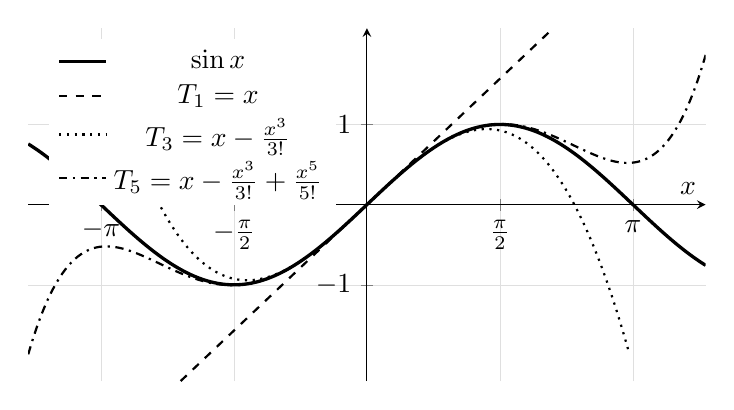
\begin{tikzpicture}
\begin{axis}[
    width=0.84\textwidth,
    height=0.50\textwidth,
    xmin=-4, xmax=4,
    ymin=-2.2, ymax=2.2,
    axis lines=middle,
    xlabel={\(x\)},
    ylabel={},
    xtick={-3.1416,-1.5708,0,1.5708,3.1416},
    xticklabels={\(-\pi\),\(-\frac{\pi}{2}\),\(0\),\(\frac{\pi}{2}\),\(\pi\)},
    ytick={-1,0,1},
    grid=both,
    grid style={line width=.1pt, draw=gray!25},
    legend style={draw=none, at={(0.03,0.97)}, anchor=north west}
]
\addplot[very thick, domain=-4:4, samples=250] {sin(deg(x))};
\addlegendentry{\(\sin x\)}
\addplot[thick, dashed, domain=-2.2:2.2, samples=150] {x};
\addlegendentry{\(T_1=x\)}
\addplot[thick, dotted, domain=-3.1:3.1, samples=180] {x - x^3/6};
\addlegendentry{\(T_3=x-\frac{x^3}{3!}\)}
\addplot[thick, dashdotted, domain=-4:4, samples=220] {x - x^3/6 + x^5/120};
\addlegendentry{\(T_5=x-\frac{x^3}{3!}+\frac{x^5}{5!}\)}
\end{axis}
\end{tikzpicture}
\caption{Taylor polynomials approximate \(\sin x\) best near their center \(0\).}
\label{fig:technology-taylor-polynomials-sine}
\end{figure}

A Python plot uses the same formulas:

\begin{verbatim}
import math
import matplotlib.pyplot as plt

def T1(x):
    return x

def T3(x):
    return x - x**3 / math.factorial(3)

def T5(x):
    return x - x**3 / math.factorial(3) + x**5 / math.factorial(5)

x_values = [ -4 + 8*j/400 for j in range(401) ]

plt.plot(x_values, [math.sin(x) for x in x_values], label="sin x")
plt.plot(x_values, [T1(x) for x in x_values], label="T1")
plt.plot(x_values, [T3(x) for x in x_values], label="T3")
plt.plot(x_values, [T5(x) for x in x_values], label="T5")

plt.ylim(-2.2, 2.2)
plt.legend()
plt.show()
\end{verbatim}

The plot should not be read as proof that the Taylor series converges.  It is visual
evidence.  Taylor's theorem gives the error estimate.

\subsection{A Taylor-series calculator}
\label{appsubsec:taylor-series-calculator}

A finite Taylor polynomial can be used as a calculator.

For example, for \(\sin x\),

\[
\sin x
=
x-\frac{x^3}{3!}+\frac{x^5}{5!}-\frac{x^7}{7!}+\cdots.
\]

The following function computes the Maclaurin polynomial through the term
\(x^{2N+1}\):

\begin{verbatim}
import math

def sin_taylor(x, N):
    total = 0.0
    for n in range(N + 1):
        term = (-1)**n * x**(2*n + 1) / math.factorial(2*n + 1)
        total += term
    return total

for N in [0, 1, 2, 3, 4]:
    approx = sin_taylor(1.0, N)
    print(N, approx, abs(approx - math.sin(1.0)))
\end{verbatim}

For \(x=1\), the series is alternating with decreasing term sizes.  The alternating error
estimate says that the error is at most the first omitted term:

\[
\left|\sin 1-\sum_{n=0}^{N}(-1)^n\frac{1^{2n+1}}{(2n+1)!}\right|
\le
\frac{1^{2N+3}}{(2N+3)!}.
\]

So the code can be paired with a proof-based error bound.

\begin{quote}
\textbf{Computing principle.}
A decimal answer becomes more valuable when it comes with a reason to trust the
digits.
\end{quote}

\section{Practice problems}
\label{appsec:technology-practice-problems}

\subsection*{Graphing windows}

\begin{enumerate}
\item The graph of
\[
f(x)=x^3-6x
\]
is shown only in the window
\[
-1\le x\le1,\qquad -6\le y\le6.
\]
Explain why this window does not show the full shape of the graph.

\item A calculator graphs
\[
g(x)=\frac{x^2-4}{x-2}
\]
as a straight line.  What feature might the graph be hiding?

\item Find a viewing window that shows both local extrema of
\[
f(x)=x^3-3x.
\]

\item Explain why a graph of
\[
y=\sin(100x)
\]
may be misleading if too few sample points are used.

\item A graphing tool connects points across a vertical asymptote.  What algebraic or
calculus information should you check?
\end{enumerate}

\subsection*{Numerical precision and roundoff}

\begin{enumerate}
\item Explain why
\[
\frac{\sqrt{1+x}-1}{x}
\]
can be numerically unstable for \(x\) near \(0\).

\item Rewrite
\[
\frac{\sqrt{1+x}-1}{x}
\]
in a more stable form for \(x\neq0\).

\item In exact arithmetic,
\[
(10^{16}+1)-10^{16}=1.
\]
Why might a finite-precision machine fail to return \(1\)?

\item In a difference quotient
\[
\frac{f(a+h)-f(a)}{h},
\]
what happens if \(h\) is too large?  What can happen if \(h\) is too small?

\item Describe the difference between truncation error and roundoff error.
\end{enumerate}

\subsection*{Calculator and CAS syntax}

\begin{enumerate}
\item What expression is represented by
\[
\texttt{1/x+1}?
\]
How should you type
\[
\frac1{x+1}?
\]

\item In Python, what is wrong with typing
\[
\texttt{x\string^2}
\]
if you intend \(x^2\)?

\item Explain the difference between
\[
\texttt{exp(-x**2)}
\]
and
\[
\texttt{exp(-x)**2}.
\]

\item Why should a calculator be in radian mode when checking
\[
\frac{d}{dx}\sin x=\cos x?
\]

\item A CAS returns
\[
\log(x)
\]
for
\[
\int \frac1x\,dx.
\]
What real-domain issue should you remember?
\end{enumerate}

\subsection*{Simple Python experiments}

\begin{enumerate}
\item Write Python code to compute
\[
\frac{(2+h)^2-2^2}{h}
\]
for
\[
h=1,\ 0.1,\ 0.01,\ 0.001.
\]
What value do the results approach?

\item Modify the bisection code to find a root of
\[
f(x)=x^2-2
\]
on \([1,2]\).

\item Use the midpoint rule to approximate
\[
\int_0^1 x^2\,dx
\]
with \(n=10\).  Compare with the exact value.

\item Use Euler's method with step size \(h=0.1\) to approximate the solution of
\[
y'=y,\qquad y(0)=1
\]
at \(t=1\).

\item Use Newton's method to approximate \(\sqrt2\) by applying the method to
\[
f(x)=x^2-2.
\]
\end{enumerate}

\subsection*{Plotting sequences, sums, and Taylor polynomials}

\begin{enumerate}
\item Plot the first \(30\) terms of
\[
a_n=\frac{n}{n+1}.
\]
What limit does the plot suggest?

\item Compute and plot the partial sums of
\[
\sum_{k=1}^{\infty}\frac1{k^2}
\]
for \(1\le n\le100\).  Do the partial sums appear to settle?

\item Compute and plot the partial sums of the harmonic series
\[
\sum_{k=1}^{\infty}\frac1k
\]
for \(1\le n\le1000\).  Why can the plot be misleading?

\item Plot
\[
\sin x,
\qquad
T_1(x)=x,
\qquad
T_3(x)=x-\frac{x^3}{3!},
\qquad
T_5(x)=x-\frac{x^3}{3!}+\frac{x^5}{5!}
\]
on \([-4,4]\).  Where do the Taylor polynomials give the best approximation?

\item For
\[
e^x=\sum_{n=0}^{\infty}\frac{x^n}{n!},
\]
write code to compute the Maclaurin polynomial
\[
T_N(x)=\sum_{n=0}^{N}\frac{x^n}{n!}.
\]
Compare \(T_N(1)\) with \(e\) for \(N=1,2,3,4,5,10\).
\end{enumerate}

\section*{Answers to Appendix E practice problems}
\label{ans:appendix-e-practice}

\subsection*{Graphing windows}

\begin{enumerate}
\item
The window \([-1,1]\) in \(x\) does not include the critical points of
\[
f(x)=x^3-6x.
\]
Since
\[
f'(x)=3x^2-6=3(x^2-2),
\]
the critical points are
\[
x=\pm\sqrt2\approx \pm1.414.
\]
They lie outside the small window.  A wider window such as \([-3,3]\) shows the
rise-fall-rise behavior.

\item
\[
g(x)=\frac{x^2-4}{x-2}
=
\frac{(x-2)(x+2)}{x-2}
=
x+2,
\qquad x\neq2.
\]
The graph is the line \(y=x+2\) with a hole at
\[
(2,4).
\]

\item
For
\[
f(x)=x^3-3x,
\]
we have
\[
f'(x)=3x^2-3=3(x-1)(x+1).
\]
So the critical points are
\[
x=-1,\qquad x=1.
\]
A window such as
\[
-2.5\le x\le2.5,
\qquad
-4.5\le y\le4.5
\]
shows both local extrema.

\item
The function \(\sin(100x)\) oscillates rapidly.  If the graphing tool samples too few
points, it may miss peaks and troughs between sample points and draw a misleading
connected curve.

\item
Check where the denominator is zero, compute one-sided limits, and identify vertical
asymptotes.  The graph should not be trusted across inputs where the function is
undefined.
\end{enumerate}

\subsection*{Numerical precision and roundoff}

\begin{enumerate}
\item
For \(x\) near \(0\), the two numbers
\[
\sqrt{1+x}
\quad\text{and}\quad
1
\]
are very close.  Subtracting nearly equal stored numbers can lose significant digits.

\item
Rationalize:
\[
\frac{\sqrt{1+x}-1}{x}
\cdot
\frac{\sqrt{1+x}+1}{\sqrt{1+x}+1}
=
\frac{1}{\sqrt{1+x}+1},
\qquad x\neq0.
\]

\item
A finite-precision machine may not store \(10^{16}+1\) distinctly from \(10^{16}\).
If both are stored as the same floating-point number, their computed difference is \(0\),
not \(1\).

\item
If \(h\) is too large, the secant slope may be a poor approximation to the tangent
slope.  This is truncation error.  If \(h\) is too small, the subtraction
\[
f(a+h)-f(a)
\]
may lose significant digits.  This is roundoff error.

\item
Truncation error comes from replacing an infinite or limiting process by a finite one.
Roundoff error comes from storing and computing with finitely many digits.
\end{enumerate}

\subsection*{Calculator and CAS syntax}

\begin{enumerate}
\item
\[
\texttt{1/x+1}
\]
means
\[
\frac1x+1.
\]
To type
\[
\frac1{x+1},
\]
use
\[
\texttt{1/(x+1)}.
\]

\item
In ordinary Python numerical code, \texttt{\string^} is not exponentiation.  Use
\[
\texttt{x**2}.
\]

\item
\[
\texttt{exp(-x**2)}
\]
means
\[
e^{-x^2}.
\]
But
\[
\texttt{exp(-x)**2}
\]
means
\[
(e^{-x})^2=e^{-2x}.
\]

\item
The derivative formula
\[
(\sin x)'=\cos x
\]
is true when \(x\) is measured in radians.  Degree mode changes the scale of the input
and therefore changes the numerical derivative.

\item
For real-valued calculus,
\[
\int \frac1x\,dx=\ln|x|+C.
\]
A CAS output of \(\log(x)\) usually assumes \(x>0\), or it is working in a context
where branch choices are being handled differently.
\end{enumerate}

\subsection*{Simple Python experiments}

\begin{enumerate}
\item
The quotient is
\[
\frac{(2+h)^2-2^2}{h}=4+h.
\]
For
\[
h=1,\ 0.1,\ 0.01,\ 0.001,
\]
the values are
\[
5,\quad 4.1,\quad 4.01,\quad 4.001.
\]
They approach \(4\).

\item
Use the same bisection structure with

\begin{verbatim}
def f(x):
    return x**2 - 2

left = 1.0
right = 2.0
\end{verbatim}

The midpoint values approach

\[
\sqrt2\approx1.41421356.
\]

\item
For \(f(x)=x^2\) on \([0,1]\), the exact value is

\[
\int_0^1 x^2\,dx=\frac13.
\]

The midpoint rule with \(n=10\) uses

\[
\Delta x=0.1
\]

and midpoints

\[
0.05,\ 0.15,\ldots,\ 0.95.
\]

The approximation is

\[
M_{10}=0.3325.
\]

It is close to

\[
\frac13\approx0.333333.
\]

\item
Euler's method for

\[
y'=y,\qquad y(0)=1
\]

with \(h=0.1\) uses

\[
y_{n+1}=y_n+0.1y_n=1.1y_n.
\]

After \(10\) steps,

\[
y_{10}=1.1^{10}\approx2.593742.
\]

The exact value is

\[
e^1=e\approx2.718282.
\]

\item
For

\[
f(x)=x^2-2,
\qquad
f'(x)=2x,
\]

Newton's method is

\[
x_{n+1}
=
x_n-\frac{x_n^2-2}{2x_n}
=
\frac12\left(x_n+\frac2{x_n}\right).
\]

Starting with \(x_0=1.5\), the iterates quickly approach

\[
\sqrt2\approx1.41421356.
\]
\end{enumerate}

\subsection*{Plotting sequences, sums, and Taylor polynomials}

\begin{enumerate}
\item
\[
a_n=\frac{n}{n+1}=1-\frac1{n+1}.
\]
The plot should suggest

\[
a_n\to1.
\]

\item
The partial sums of

\[
\sum_{k=1}^{\infty}\frac1{k^2}
\]

increase and appear to settle.  The series converges.  Its exact sum is

\[
\frac{\pi^2}{6},
\]

though that exact result is beyond the usual first test for convergence.

\item
The harmonic partial sums grow very slowly.  A plot up to \(n=1000\) may look as if
the sums are settling, but the harmonic series diverges.  This is a classic example where
numerical evidence can mislead.

\item
The Taylor polynomials give the best approximation near the center

\[
x=0.
\]

Farther from \(0\), low-degree Taylor polynomials become less reliable.

\item
The code should compute

\[
T_N(1)=\sum_{n=0}^{N}\frac1{n!}.
\]

As \(N\) increases, these values approach

\[
e\approx2.718281828.
\]

For example,

\[
T_1(1)=2,
\]

\[
T_2(1)=2.5,
\]

\[
T_3(1)=2.666\ldots,
\]

and

\[
T_{10}(1)
\]

is already very close to \(e\).
\end{enumerate}